\subsection{Définition des constantes et macro}

L'utilisation de constante nous permet de modifier plus simplement des
éléments clefs du jeu. Pour cela nous utilisons les constantes suivantes
:  
\begin{itemize}
\item {\textit{NB\_JOUEURS}} : Nous permet de modifier le nombre de
  joueur en théorie.
\item {\textit{NB\_LIGNES}} : Nous permet de modifier le nombre de
  ligne dans la grille de notre jeu.
\item {\textit{NB\_COLONNES}} : Nous permet de modifier le nombre de
  colonne dans la grille de notre jeu.
\item {\textit{NB\_BATALS}} : Nous permet de modifier le nombre de
  bateau dans le jeu.
\item {\textit{NB\_MONSTRES}} : Nous permet de modifier le nombre de
  monstre en théorie (cf : ACHIEVEMENT3).
\item {\textit{NB\_PIXEL\_CASE}} : Nous permet de modifier la taille
  d'une case dans la représentation graphique en SDL.
\item {\textit{TAILLE\_MAX\_BAT}} : C'est la taille maximale qu'un
  bateau peut avoir, elle nous permet de pouvoir initialiser la
  structure Batal et Joueur.
\item {\textit{TAB\_TAILLE}} : Cette constante nous permet d'obtenir un tableau d'entier où chaque entier représente la taille du bateau d'indice i du tableau.
\end{itemize}
On utilise aussi une macro qui nous permet de mettre de la couleur
dans le terminal.

\subsection{Définition des structures}

\subsubsection{Position}
Cette structure nous permet de nous repérer dans la grille, elle contient : 
\begin{itemize}
\item Un entier qui correspond à la ligne
\item Un entier qui correspond à la colonne
\end{itemize}

\subsubsection{Case}

Cette structure nous permet de savoir l'état d'une position de la grille, elle contient :
\begin{itemize}
\item Un tableau d'entier où l'indice 0 correspond à une case qui
  est oblitérée ou non (-1 : oblitérée, 0 : intact) et l'indice 1 à
  {\textit{NB\_JOUEURS}} permet de savoir si un bateau du joueur est dans
  cette case (1 : présent, 0 : absent) et de même pour le monstre
  à l'indice {\textit{NB\_JOUEURS}} + 1 (1 : présent, 0 : absent)
\end{itemize}

\subsubsection{Grille}

Cette structure permet de représenter la grille du jeu, elle contient
:
\begin{itemize}
\item Un tableau de {\textit{NB\_LIGNES}} * {\textit{NB\_COLONNES}}
  Cases pour représenter entièrement notre grille.
\end{itemize}

\subsubsection{Alignement}
Cette énumération nous permet d'associer à chaque bateau une forme et/ou un alignement, par exemple savoir si le bateau est horizontal, si le bateau est vertical, si le bateau est en O, en H, ou en L dans une certaine orientation. Il faut savoir que les bateaux linéaires horizontaux ou verticaux peuvent avoir une taille quelconque tant que celle-ci ne dépasse pas le nombre de lignes de la grille pour le batal vertical ou le nombre de colonnes pour le batal horizontal. Si le bateau est en O, alors nécessairement, il aura une taille de 8, s'il est en H, il aura une taille de 7 et s'il est en L, une taille de 4. Voici un schéma associant chaque nombre de l'énumération à un type de bateau. 
\begin{flushleft}
\begin{tabular}[t]{|c|c|c|c|c|}
  \hline
  & & & &  \\
  \hline
  & & & &  \\
  \hline
  & \cellcolor{blue} & \cellcolor{blue} & \cellcolor{blue} &   \\
  \hline
  & & & &  \\
  \hline
  & & & &  \\
  \hline
  \multicolumn{5}{c}{Enum 1}\\
\end{tabular}
\hspace{3cm}
\begin{tabular}[t]{|c|c|c|c|c|}
  \hline
  & & & &  \\
  \hline
  & & \cellcolor{blue} & &  \\
  \hline
  & & \cellcolor{blue} & &  \\
  \hline
  & & \cellcolor{blue} & &  \\
  \hline
  & & & &  \\
  \hline
  \multicolumn{5}{c}{Enum 10}\\
\end{tabular}
\hspace{3cm}
\begin{tabular}[t]{|c|c|c|c|c|}
  \hline
  & & & &  \\
  \hline
  & \cellcolor{blue}& \cellcolor{blue}& \cellcolor{blue}&  \\
  \hline
  & \cellcolor{blue}& & \cellcolor{blue}&  \\
  \hline
  & \cellcolor{blue}& \cellcolor{blue}& \cellcolor{blue}&  \\
  \hline
  & & & &  \\
  \hline
  \multicolumn{5}{c}{Enum 20}\\
\end{tabular}
\end{flushleft}
\begin{flushleft}
\begin{tabular}[t]{|c|c|c|c|c|}
  \hline
  & & & &  \\
  \hline
  & \cellcolor{blue}& & \cellcolor{blue}&  \\
  \hline
  & \cellcolor{blue} &\cellcolor{blue}  & \cellcolor{blue} &   \\
  \hline
  & \cellcolor{blue}& &\cellcolor{blue} &  \\
  \hline
  & & & &  \\
  \hline
  \multicolumn{5}{c}{Enum 31}\\
\end{tabular}
\hspace{3cm}
\begin{tabular}[t]{|c|c|c|c|c|}
  \hline
  & & & &  \\
  \hline
  & \cellcolor{blue}&  \cellcolor{blue}& \cellcolor{blue}&  \\
  \hline
  & & \cellcolor{blue} & &  \\
  \hline
  &\cellcolor{blue} & \cellcolor{blue} & \cellcolor{blue} &  \\
  \hline
  & & & &  \\
  \hline
  \multicolumn{5}{c}{Enum 32}\\
\end{tabular}
\hspace{3cm}
\begin{tabular}[t]{|c|c|c|c|c|}
  \hline
  & & & &  \\
  \hline
  & \cellcolor{blue}& & &  \\
  \hline
  &  \cellcolor{blue}&  &  &   \\
  \hline
  & \cellcolor{blue}& \cellcolor{blue}& &  \\
  \hline
  & & & &  \\
  \hline
  \multicolumn{5}{c}{Enum 41}\\
\end{tabular}
\end{flushleft}
\begin{flushleft}
\begin{tabular}[t]{|c|c|c|c|c|}
  \hline
  & & & &  \\
  \hline
  & & \cellcolor{blue}& &  \\
  \hline
  & &  \cellcolor{blue}&  &   \\
  \hline
  & \cellcolor{blue}& \cellcolor{blue}& &  \\
  \hline
  & & & &  \\
  \hline
  \multicolumn{5}{c}{Enum 42}\\
\end{tabular}
\hspace{3cm}
\begin{tabular}[t]{|c|c|c|c|c|}
  \hline
  & & & &  \\
  \hline
  & \cellcolor{blue}&  \cellcolor{blue}& &  \\
  \hline
  & \cellcolor{blue}&  & &  \\
  \hline
  & \cellcolor{blue}&  & &  \\
  \hline
  & & & &  \\
  \hline
  \multicolumn{5}{c}{Enum 43}\\
\end{tabular}
\hspace{3cm}
\begin{tabular}[t]{|c|c|c|c|c|}
  \hline
  & & & &  \\
  \hline
  & \cellcolor{blue}& \cellcolor{blue} & &  \\
  \hline
  & & \cellcolor{blue} & &  \\
  \hline
  & &  \cellcolor{blue}& &  \\
  \hline
  & & & &  \\
  \hline
  \multicolumn{5}{c}{Enum 44}\\
\end{tabular}
\end{flushleft}
\begin{flushleft}
\begin{tabular}[t]{|c|c|c|c|c|}
  \hline
  & & & &  \\
  \hline
  & & & \cellcolor{blue}&  \\
  \hline
  & \cellcolor{blue} &  \cellcolor{blue}& \cellcolor{blue} &   \\
  \hline
  & & & &  \\
  \hline
  & & & &  \\
  \hline
  \multicolumn{5}{c}{Enum 45}\\
\end{tabular}
\hspace{3cm}
\begin{tabular}[t]{|c|c|c|c|c|}
  \hline
  & & & &  \\
  \hline
  &\cellcolor{blue} & \cellcolor{blue} &\cellcolor{blue} &  \\
  \hline
  & &  &\cellcolor{blue} &  \\
  \hline
  & &  & &  \\
  \hline
  & & & &  \\
  \hline
  \multicolumn{5}{c}{Enum 46}\\
\end{tabular}
\hspace{3cm}
\begin{tabular}[t]{|c|c|c|c|c|}
  \hline
  & & & &  \\
  \hline
  & \cellcolor{blue}&  & &  \\
  \hline
  & \cellcolor{blue}&\cellcolor{blue} &\cellcolor{blue} &  \\
  \hline
  & &  & &  \\
  \hline
  & & & &  \\
  \hline
  \multicolumn{5}{c}{Enum 47}\\
\end{tabular}
\end{flushleft}
\hspace{5.32cm}
  \begin{tabular}[t]{|c|c|c|c|c|}
  \hline
  & & & &  \\
  \hline
  & \cellcolor{blue}&\cellcolor{blue} &\cellcolor{blue} &  \\
  \hline
  & \cellcolor{blue}&  & &  \\
  \hline
  & &  & &  \\
  \hline
  & & & &  \\
  \hline
  \multicolumn{5}{c}{Enum 48}\\
  \end{tabular}
\subsubsection{Batal}

Cette structure nous permet de représenter un bateau dans le jeu, elle
contient :
\begin{itemize}
\item Un entier qui représente la taille du bateau
\item Un tableau de Position correspondant à toutes les positions
  que le bateau occupe
\item Un entier qui représente l'alignement 
\item Un entier qui représente à quelle joueur appartient le bateau
\end{itemize}

\subsubsection{Joueur}

Cette structure nous permet de rassembler toutes les informations
concernant un joueur, elle contient :
\begin{itemize}
\item Un entier qui représente le numéro du joueur
\item Un tableau de Batal
\item Un tableau de Position correspondant à toutes les cases des
  bateaux qui ne sont pas encore oblitérées
\item Un entier qui correspond au nombre de Position qui sont encore
  en vie (taille courante du tableau précédent).
\end{itemize}

\subsection{Fonctionnement achievement0}

\subsubsection{Fonctions et Complexité}

\begin{itemize}

\item Les fonctions commençant par init:
\begin{lstlisting} 
void init_grille(struct Grille *grille)
void init_batal(struct Batal *joueur, int taille, struct Position *positon, int alignement, int nbjoueur)
void init_rond(struct Batal *bateau, struct Position *posinit)
void init_H(struct Batal *bateau,struct Position *posinit,int alignement)
void init_L(struct Batal *bateau,struct Position *posinit,int alignement)
void init_joueur(struct Joueur *joueur, int nbjoueur)
\end{lstlisting}
Ces fonctions vont permettre d'initialiser les différents éléments nécessaire au jeu et à la baseline. \textit{init\_grille} est de complexité linéaire en $\Theta(n)$ avec n le nombre de case de la grille. De même, \textit{init\_batal} est de complexité linéaire en $\Theta(n)$ avec n la taille du bateau initialisé.\\

\item Les fonctions \textit{placer\_batal} et \textit{verif\_pour\_mettre\_bateau}:
\begin{lstlisting} 
int verif_pour_mettre_bateau(struct Grille *grille, struct Batal *bateau)
void placer_batal(struct Grille *grille, struct Batal *bateau)
\end{lstlisting}
Ces deux fonctions permettent de placer un bateau et d'être sur que le bateau se situe bien dans la grille, dans de bonnes positions. Le principe est simple, on choisit aléatoirement une position initiale et une forme à l'aide des fonctions \textit{position\_aléatoire} et \textit{alignement\_aléatoire} et à partir de cette première case, la fonction \textit{placer\_batal} va placer le bateau si la fonction \textit{verif\_pour\_mettre\_bateau} retourne 1 pour dire que c'est possible, sinon on recommence le processus.\\
La fonction \textit{verif\_pour\_mettre\_bateau} est de complexité $\Theta(n)$ où n est la taille du bateau à vérifier.\\
\item Les fonctions pour afficher:\\
Deux affichages sont possibles pour la grille de jeu:
\begin{itemize}
\item Un affichage en texte dans la fenêtre du terminal avec la fonction \textit{afficher\_grille}, voici un exemple en image:\\
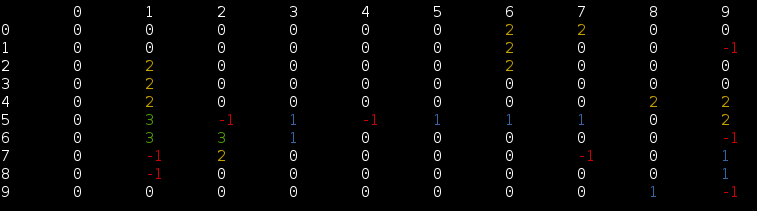
\includegraphics[scale=0.7]{image/grille_console.png}

La légende est la suivante:

\begin{itemize}
\item Le chiffre \textcolor{red}{-1} correspond à une case oblitérée.
\item Le chiffre 0 correspond à une case vide et non oblitérée.
\item Le chiffre \textcolor{blue}{1} correspond à une case occupée par un batal du joueur 1.
\item Le chiffre \textcolor{orange}{2} correspond à une case occupée par un batal du joueur 2.
\item Le chiffre \textcolor{ForestGreen}{3} correspond à une case occupée simultanément par un batal du joueur 1 et par un batal du joueur 2.
\end{itemize}

\item Un affichage en SDL dans une nouvelle fenêtre avec la fonction \textit{afficher\_grille\_SDL}, voici un exemple en image:\\

\begin{center}
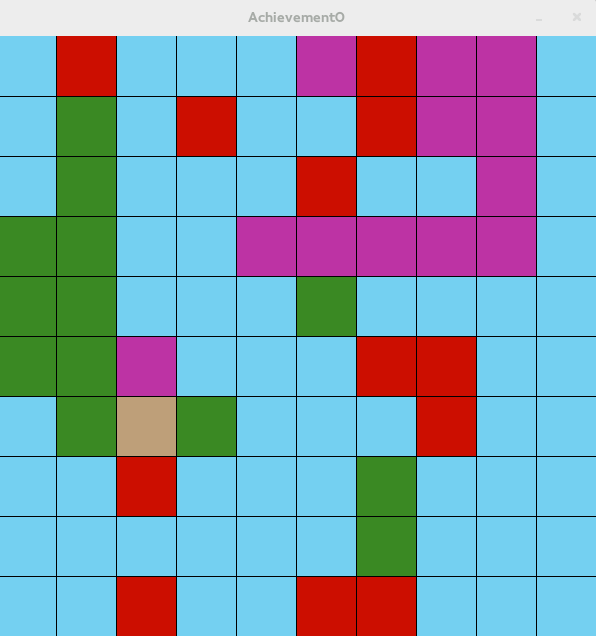
\includegraphics[scale=0.6]{image/grille_SDL.png}
\end{center}

La légende est la suivante:

\begin{itemize}
\item Les cases \textcolor{SkyBlue}{bleues} correspondent à des cases vides et non oblitérées.
\item Les cases \textcolor{red}{rouges} correspondent à des cases oblitérées.
\item Les cases \textcolor{ForestGreen}{vertes} correspondent à des cases occupées par un batal du joueur 1.
\item Les cases \textcolor{Mulberry}{violettes} correspondent à des cases occupées par un batal du joueur 2.
\item Les cases \textcolor{Tan}{beige} correspondent à des cases occupées simultanément par un batal du joueur 1 et par un batal du joueur 2.
\end{itemize}

\end{itemize}
La complexité pour les fonctions d'affichage sont de complexité linéaire en $\Theta(n)$, avec n le nombre de cases de la grille.


\item Les fonctions aléatoires:
\begin{lstlisting} 
void melange_tab();
struct Position position_aleatoire()
int alignement_aleatoire(int taille)
\end{lstlisting}
Ces trois fonctions utilisent la fonction \textit{rand} pour ainsi respectivement mélanger le tableau des positions pour obtenir ainsi plus rapidement des positions aléatoires pour une partie, retourner une position aléatoire, retourner un alignement aléatoire.

\end{itemize}

\subsubsection{Fonctionnement global du jeu}
\begin{lstlisting}
  init_grille(&grille);
  init_joueur(&joueur1, 1);
  init_joueur(&joueur2, 2);
  init_tab();
  melange_tab();
  placer_batal_joueur(&joueur1, &grille);
  placer_batal_joueur(&joueur2, &grille);
  afficher(&grille, ecran, 1, affichage);
  while(un_bateau_toujours_en_vie(&grille, &joueur1) && un_bateau_toujours_en_vie(&grille, &joueur2)){
    pos = TAB_POSITION[indice];
    obliterer_une_case(&grille, &pos, &joueur1, &joueur2);
    indice ++;
    pos = TAB_POSITION[indice];
    obliterer_une_case(&grille, &pos, &joueur1, &joueur2);
    indice ++;
    afficher(&grille, ecran, 1, affichage);
  }
  if(un_bateau_toujours_en_vie(&grille, &joueur1)){
    return(1);
    }
  if(un_bateau_toujours_en_vie(&grille, &joueur2)){
    return(2);
  }
  return(0);
\end{lstlisting}
Voici le code C permettant de simuler une partie, tout d'abord on initialise toutes nos structures utiles à la partie: 2 joueurs, la grille. Ensuite, on relie les deux grâce à la fonction \textit{placer\_batal\_joueur} qui va en même temps initialiser nos bateaux pour les deux joueurs en les plaçant à des positions possibles. Pour finir l'initialisation, on affiche pour la première fois la grille. C'est à partir de la boucle \textbf{while} que commence la partie, la fonction \textit{un\_bateau\_toujours\_en\_vie} va savoir si les joueurs sont encore en jeu (avec une case de leurs bateaux non oblitérées) ou non (toutes leurs cases oblitérées), d'où l'utilisation de cette fonction comme condition pour la boucle \textbf{while}. Ensuite, on prend, les unes après les autres, les cases du tableau de positions mélanger initialement et chaque joueur oblitère une case avec la fonction \textit{obliterer\_une\_case}. \\
On peut justifier que la boucle se termine:\\
Posons $N=NB\_COLONNES*NB\_LIGNES$ et $i=indice$, on a donc pour variant de boucle $N-i$ puisqu'une fois que toutes cases sont parcourues (dans le pire des cas), obligatoirement il n'y a plus de joueurs en jeu.\\

\subsection{Problèmes rencontrés}
Nous avons rencontrés 2 problèmes dans ce premier achievement qui sont les suivants:\\
\begin{itemize}
\item Un problème avec la fonction \textit{rand} puisqu'à chaque fois sa valeur valait la même chose. On a donc inclus en plus de la bibliothèque \textit{stdlib.h}, la bibliothèque \textit{time.h} qui permet à partir de la fonction \textit{srand} d'initialiser la fonction \textit{rand}. De plus, nous avons fait une fonction \textit{init\_rand} qui initialise avec l'appel de \textit{srand} la fonction \textit{rand} et ainsi on a donc un moyen d'obtenir un nombre aléatoire beaucoup plus efficace qu'avec la fonction \textit{rand} seulement. De même, si nous utilisons un tableau de positions que nous mélangeons au départ c'est pour un gain de temps car il n'est pas possible de retomber plusieurs fois de suite sur la même position avec cette technique.\\

\item Le deuxième problème a été de se projeter dans les futurs étapes (achievements) du projet, imaginer la mise en place de bateau en O, H ou L directement dans cet achievement, la possibilité de changer la taille des bateaux, de changer le nombre de bateaux. Nous avons donc, dans le but d'un gain d'efficacité pour les achievements suivants, essayé de mettre en place des structures et des stratégies pour gérer les futurs requêtes du jeu. 
\end{itemize}


